\chapter{Background} \label{chap:background}
% -------------------------
%% QUOTE
\vspace*{\fill}
\epigraph{The more we learn about the world, and the deeper our learning, the more conscious, specific, and articulate will be our knowledge of what we do not know, our knowledge of our ignorance.\\ For this, indeed, is the main source of our ignorance — the fact that\\ \textbf{our knowledge can be only finite, while our ignorance must necessarily be infinite.}}%
{\textit{Conjectures and Refutations (1963)}\\ \textsc{Karl Popper}}
\clearpage{\thispagestyle{empty}\cleardoublepage}
%%
%% Body of the chapter
%%%%%%%%%%%%%%%%%%%%%%
\section{Nanoparticles and Nanomaterials}
If we assumed a range for all the sizes colloids could assume, Nanoparticles would be at the smaller end of it \citep{Goodwin2009}. The different industries have, in the last decade or two, found significant applications for nanoparticles in manufacturing products with special characteristics. In all these applications, the small size of nanoparticles is exploited for development of new materials, tools and devices. Generally speaking, ``nanoparticles" are particles whose dimensions (at least one dimension) are smaller than 100 nm. At these lengths, special electronic, thermal, mechanical and chemical properties appear (such as greater surface area per volume, higher reactivity with other molecules), the application of which can enable a plethora of new solutions. Figure \ref{cht:NPsurfaceVolume} shows surface area to volume ratio of the same volume of materials in ranges of millimeter, micrometer and nanometer. As illustrated by \citet{Amanullah2009}, conversion of a particle from the millimeter scale to the nanometer scale will multiply its area to volume ratio a million fold. 
\begin{figure}[h]
    \centering
    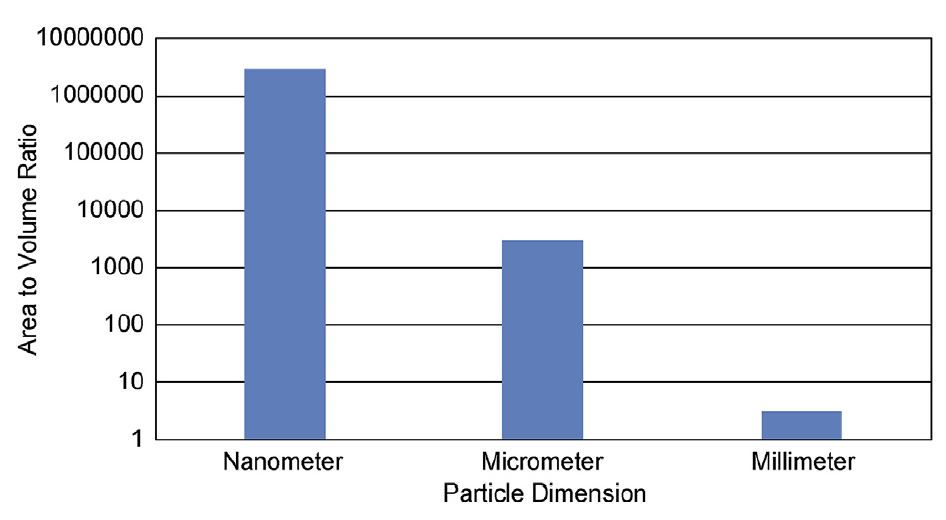
\includegraphics[width=\textwidth]{img/cht/NPsurfaceVolume.png}
    \caption{Surface area to volume ratio of the same volume of materials (adapted from \citet{Amanullah2009})}
    \label{cht:NPsurfaceVolume}
\end{figure}

\citet{Fakoya2017} definet ``Nanomaterials" as materials that are composed of nanoparticles as part of their structure. Nanomaterials inherit most of the qualities and enhanced properties from the embedded nanoparticles. Compared to regular materials, in nanomaterilas most of the atoms occupy the surface of the particles \citep{Wilson2002}. Nanomaterials are mainly produced by six common methods \citep{Hussainova2010}: electrodeposition \citep{Bera2004}, ball milling \citep{Cao2007}, chemical vapor deposition \citep{AZO2013}, plasma arcing \citep{Shashurin2015}, sol-gel synthesis \citep{Ficai2017}, and the use of natural nanoparticles \citep{Wilson2002}. 

\section{State of the art and applications of nanotechnology in the oil and gas industry}
More recently, the oil industry has started to recognize nanoparticles and nanotechnology as a potential for breakthroughs in all aspects of the industry, from exploration to drilling, from reservoir management to production \citep{Cocuzza2011}. Drilling and completion projects, for example, can benefit from specific characteristics of nanoparticles such as their mechanical strength, corrosion resistance and lightness. The exploration branch can take advantage of nano-sensors for modern monitoring techniques. And of course, reservoir engineers could apply nanotechnology to development of ``smart fluids" for water shut-off and enhanced oil recovery (EOR) purposes. 

\subsection{Drilling and hydraulic fracturing}
It is interesting to note that naturally occurring nanoparticles have played a role in the oil industry for the past 60 years. An example would be drilling muds which are composed of nanoparticles made of clays (disks of aluminosilicates) which have thicknesses in the range of 1 nm \citep{Krishnamoorti2015} and have significant rheological properties. Still, nanotechnology can play a more promising role in the oil and gas industry by development of synthetic nanoparticles. These types of nanoparticles have carefully controlled functionalities (chemical groups) attached to them, which tailors the chemical interactions, shape and size of the particles to the technical needs of the industry.

Operating conditions, in the recent years, have generally shifted towards harsher and more extreme cases. Deeper reservoirs (sometimes under deepwater environments), horizontal wells and harsh environmental conditions are a few examples. Conventional materials, fluids and cements have only a substandard performance under these conditions. With the advent of nanotechnology, drilling and production operations have benefited from the development of a new group of fluids referred to as ``smart fluids". These fluids improve the performance of said operations by altering wettablity, reducing drag and consolidating formation sand \citep{Wasan2003, Chaudhury2003, Amanullah2009}. Drilling speeds have been improved (at least in the lab scale) by treating the drilling mud with nanoparticles and superfine powders, reducing or even eliminating the damage to the near wellbore formation \citep{Esmaeili2011}.

Drilling fluids carry the cuttings in the well to the surface, while hydraulic fracturing fluids transport proppants to the fractured zones around the wellbore. Current fluids used for drilling and fracturing contain particles in the macro and micro range and therefore result in formation damage by leaving thick mud cake around the annulus. According to \citet{Outmans1958}, when there is a pressure difference between the mud column in the borehole and the formation fluid, the drill string sticks to the wall of the wellbore. This effect is referred to as ``differential sticking" and is magnified when low quality drilling muds are used. 

As a result researchers in the drilling area have continuously been looking for better solutions in the development of such fluids, and therefore nanoparticles have started to play a role in recent years. \citet{Amanullah2011} conducted several experiments on water-based muds incorporating nanomaterials. They concluded that using nanotechnology can improve the rheological properties of ``smart" drilling fluids and mitigate the effects of thick and tight mud cakes. 

During drilling operations, there comes a time when it is necessary to change mud types or perform cementing operations. In either case, it would be necessary to separate the old mud from the new mud or the cement. For this purpose, special fluids known as ``spacers" are used. For example, the residual oil-based muds (OBM) in the wellbore must be removed by the spacer to prevent costly contamination of cement \citep{VanZanten2010}. The rusults from experiments carried out by \citet{Maserati2010} indicated that nano-emulsions (emulsions where: droplet size of internal phase $<$ 500 nm) perform better than common spacers at casing - open hole cleaning and wettability alteration for better adhesion of slurry in the casing - open hole gap. 

Drilling in shale formations poses specific challenges to the operator companies. One such challenge is fluid penetration from mud into shale formations which will cause swelling and wellbore instability. In order to solve this problem, the nano-sized pore throats of the shale formation must be sealed. However, conventional drilling fluids are made of particles which are too large for this task. Here, nanoparticles can play a role as well. \citet{Sensoy2009} studied four field muds with shales from Atoka and Gulf of Mexico and investigated the effect of addition of silica nanoparticles to the muds. The nanoparticles were able to reduce the permeability of the shale by a factor of 5 to 50, and a as a result, water penetration was reduced by 98\%. Using scanning electron micrographs (SEM) they illustrated the Atoka shale after exposure to nanoparticles. As shown in Figure \ref{fig:npShale} they observed that their nanoparticles could plug small pore throats and in some cases aggregate and seal bigger ones. \citet{Cai2012}, \citet{Riley2012} and \citet{Young2013} performed similar studies for water-based muds, and \citet{Srivatsa2011} for surfactant-polymerbased muds using silica nanoparticles and confirmed the reduction in water/filterate invasion observed by \citet{Sensoy2009}.

\begin{figure}[h]
    \centering
    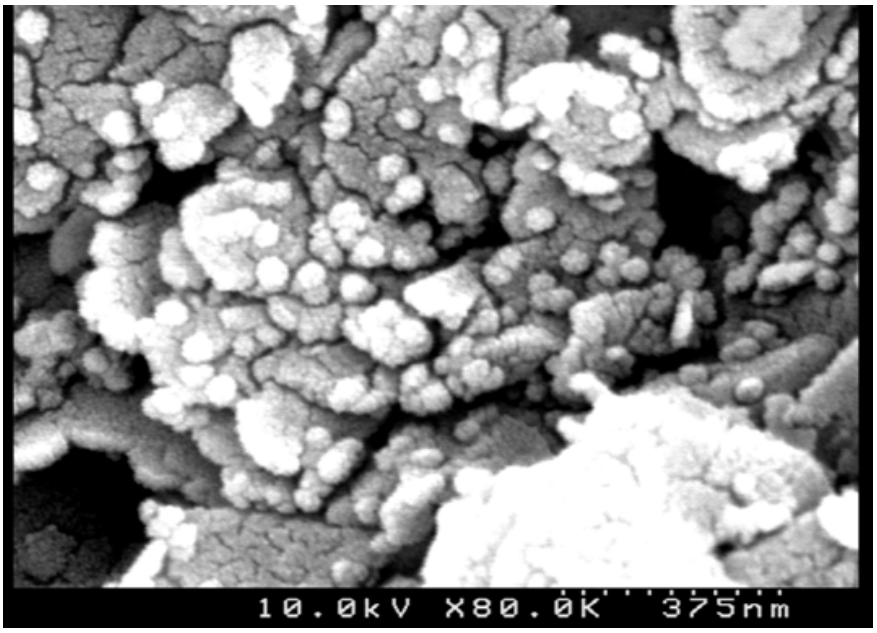
\includegraphics[width=\textwidth]{img/fig/npShale.png}
    \caption{SEM of 20 nm particles within Atoka shale (Dotted scale is 375 nm). source: \citet{Sensoy2009}}
    \label{fig:npShale}
\end{figure}

Research on nanomaterials has also found new solutions in the area of hydraulic fracturing, both for creating viscous fluids and for breaking them down. Fracturing fluids should provide sufficiently high viscosities (in the order of highly viscous gels) for transferring large amounts of proppants and creating fractures \citep{Weaver2002}. \citet{Hurnaus2015} used nanoparticles as crosslinking agents for creating viscous fluids for hydraulic fracturing with lower environmental impact. Meanwhile, \citet{Crews2010} used nanoparticle-associated surfactants in brine to develope a technology for breaking down the residual polymer from hydraulic fractures into easily producible fluids during a post-treatment stage. The resulting Viscoelastic Surfactant fluids (VES) showed crosslinked-polymer-like viscosities. These fluids contained internal breakers that broke the residual polymer without the need to contact reservoir fluids \citep{Crews2007}.

\subsection{Corrosion inhibition}
Corrosion costs the oil industry billions of dollars a year by destruction of metallic structures \citep{Brondel1994}, and it only makes sense that modern research has addressed nanomaterials as a potential agent for corrosion inhibition. 

\citet{Jauhari2011} designed a ferrofluid corrosion inhibitor composed of ferromagnetic naonparticles and studied the corrosion behavior of carbon steel in an acidic environment with various concentrations of the nanomagnetic fluid. They observed that increasing the concentration of the nanomagnetic fluid leads to an increase in the inhibition efficiency (up to an optimum concentration) and thus a reduced corrosion rate. 

The experimental resutls of \citet{Murugesan2016} revealed that Nickle based coatings, which are used for inhibiting corrosion, can be improved by the development of metal-matrix-nanocomposite coatings (MMnC). These coatings are synthesized by colliding nanoparticles with the growth surface and encapsulation of these nanoparticles by the depositing Nickle ions. Their nanocomposite coatings were able to outperform the commercially available coatings and therefore extend the lifetime of equipment which are exposed to corrosive and errosive environments. 

\subsection{Logging}
Acquiring subsurface data is inevitable, e.g., during drilling operations or later in the life cycle of a well. Logging operations are those where certain tools are run into the well with the purpose of reading representative, undisturbed and sometimes real time data about reservoir rock and fluid properties. \citet{Singh2006} claimed that an innovative system, which they called ``nanologging", could potentially provide more accurate data than logging while drilling (LWD) and measurements while drilling (MWD). In their proposed technique nanorobots are used for the purpose of logging. These robots, which are equipped with the necessary sensors, are circulated into the mud system of the borehole and at the same time they may ``swim" through the mud based on the principle of viscous forces. They would then transmit the acquired real-time data to the surface by means of an electro-magnetic transmitter. 

\subsection{Production}
Migration of formation fines is a big challenge during production operations. During production from unconsolidated reservoirs, clays and other formation fines migrate towards the production well and cause several problems such as ruining the surface and downhole equipment (in turn causing downtime and replacement costs), permeability reduction and environmental issues \citep{Tiffin1998}. \citet{Huang2008} illustrated the formation fines migration from reservoir to the near-wellbore area into the fracture proppant pack as shown in Figure \ref{fig:fines}. A comparison of Figures \ref{fig:fines1} and \ref{fig:fines2} shows how fines continue to migrate to the pack from all directions and concentrate after a while, forming larger particles and blocking the flow channels near wellbore proppant pack (in this particular case the production drops from 1000 barrels per day (bpd) to 100 bpd in only 3 months. As shown in Figure \ref{fig:fines3} this problem can be remedied by using nanoparticle-treated fracture proppant packs. The high surface enregy of the nanoparticles on the proppants will fixate the fines during production and prevent them from concentration and eventually reduction of oil rates. In recent years, a few research studies have focused on applying nanotechnology to mitigate fine migration effects \citep{Belcher2010,Habibi2011,Ogolo2012,Ahmadi2013}.

\begin{figure}[p] 
    \begin{subfigure}{.8\textwidth}
    \centering
    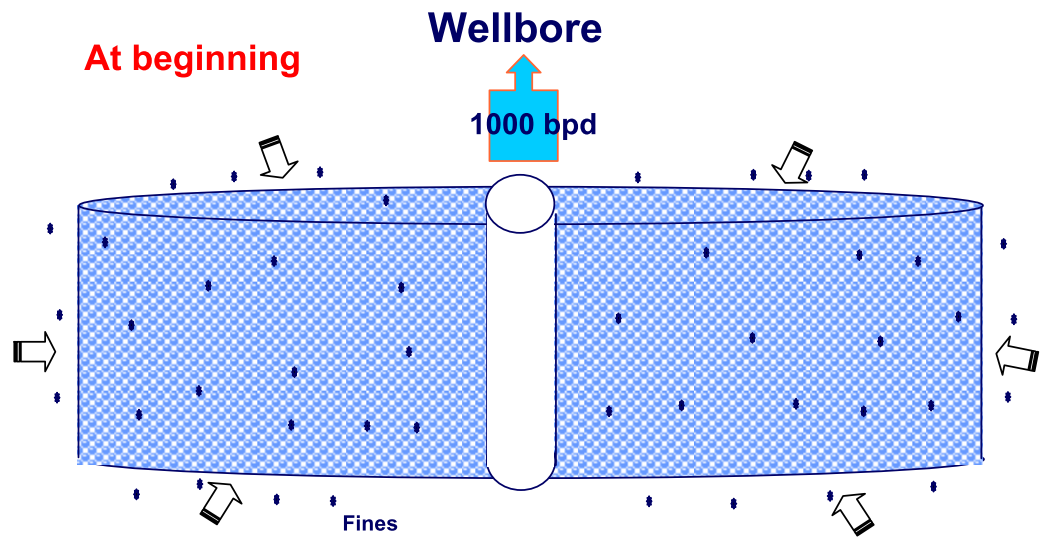
\includegraphics[width=\textwidth]{img/fig/fines1.png}
    \caption{Formation fines carried by formation fluid flow into proppant pack in all directions as well starts producing.}
    \label{fig:fines1}
    \end{subfigure}
    \\
    \begin{subfigure}{.8\textwidth}
    \centering
    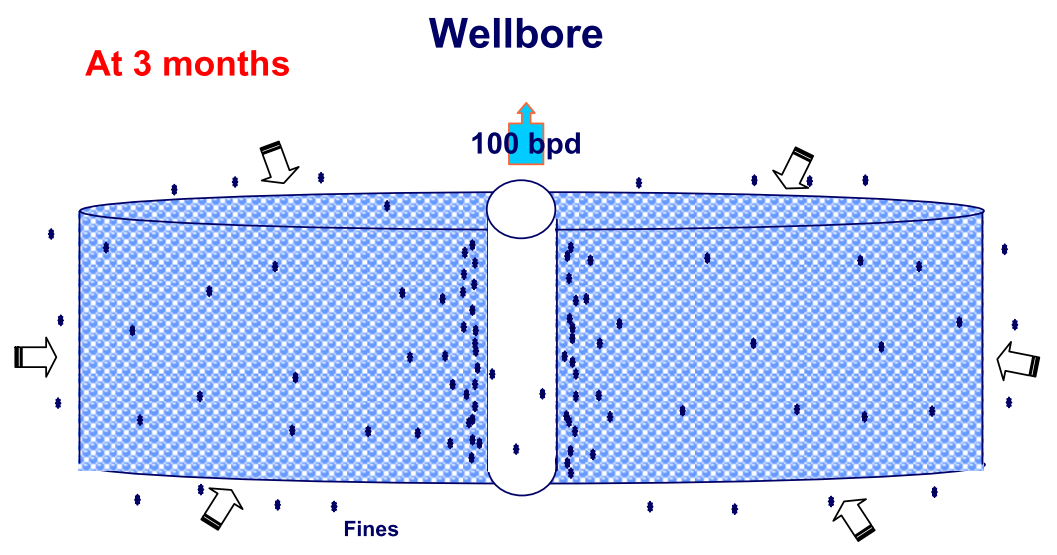
\includegraphics[width=\textwidth]{img/fig/fines2.png}
    \caption{Formation fines migration after several months of well production for non-treated proppant pack.}
    \label{fig:fines2}
    \end{subfigure}
    \\
    \begin{subfigure}{.8\textwidth}
    \centering
    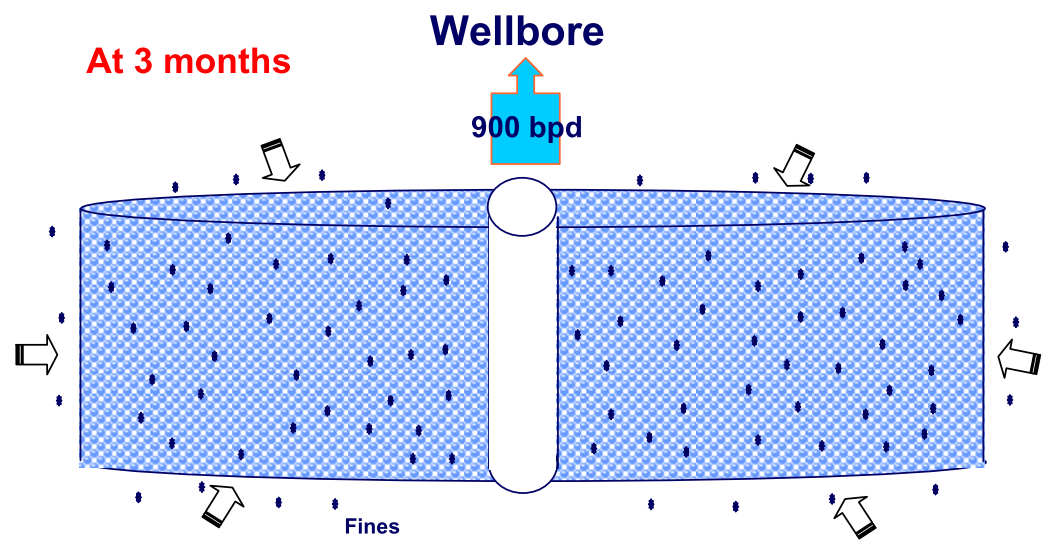
\includegraphics[width=\textwidth]{img/fig/fines3.png}
    \caption{Formation fines fixed in nanoparticle-treated proppant pack.}
    \label{fig:fines3}
    \end{subfigure}
    
    \caption{Formation fines migration. source: \citet{Huang2008}.}
    \label{fig:fines}
\end{figure}

\citet{Ogolo2013} experimentally identified magnesium oxide, aluminum oxide and zinc oxide nanoparticles as candidates for trapping unconsolidated fines. Among the candidates aluminum oxide was had the best performance, while the other two caused some permeability problems. Yet \citet{Huang2015} reported magnesium oxide nanoparticles to be performing well under water injection. They conducted experiments on stabilizing formation clays and fines during water flooding operations using nanoparticles. The results of their experiments indicated that adding 8-nm magnesium oxide particles to injection water would increase sweep efficiency by manipulating local clays and other formation fines and prevent swelling and migration of fines. 

\subsection{Enhanced Oil Recovery}
In order to benefit from nanoparticles for EOR purposes, they first need to be transported and delivered to the desired depths from the injection well within the reservoir. Accordingly, a few studies have addressed transport of nanoparticles through porous media, investigating their stability and breakthrough time in different environments. \citet{Yu2010} investigated transport and retention of aqueous dispersions of paramagnetic iron oxide nanoparticles in sedimentary reservoir rocks. Their coreflood experiments demonstrated that given the right surface coating, high concentrations of paramagnetic nanoparticles can be transported through high and low permeability rocks (Boise sandstone and Texas Cream limestone). 

In another study \citet{Yu2010a} investigated transport of carbon nanoparticles in synthetic sea water (SSW) through dolomite cores from Kuwait and Berea sandstones. The results of this study showed that high ionic strength (1 wt\% KCl) and multivalent ions (\ce{Ca^2+} and \ce{Mg^2+} grew the amount of retention that the nanoparticles experienced, and therefore delayed the breakthrough of nanoparticles dramatically. This underlying theory has been well accepted in the literature: in aqueous suspensions high ionic strength caused by high salt concentration shrinks the electric double layer and reduces the repulsion \citep{Goodwin2009, Tadros2013}. In a later study, \citet{Yu2012}investigated the transport and adsorption of silica nanoparticles in Berea sandstone, Indiana limestone, and dolomite. They observed that nanoparticles could pass through sandstone and limestone without noticeably changing the permeability. However, they could not observe the same effect in dolomite as the cores were plugged and the permeability was reduced. 

Wettability alteration is one of the major mechanisms exploited by some EOR methods. To study wettability alteration of water wet rocks obtained from the Niger Delta, \citet{Onyekonwu2010} looked into three types of polysilicon nanoparticles, namely lipophobic and hydrophilic (LHPN), hydrophobic and lipophilic (HLPN) and neutrally wet (NWPN). They reported that NWPN and HLPN dispersed in ethanol successfuly altered wettability and reduced interfacial tension, and recommended them for use in EOR for water-wet formations. \citet{Roustaei2013} evaluated the effect of modified silica nanoparticles on IFT reduction in two different Iranian light and intermediate oil reservoirs. Their results indicated more effective IFT reduction in light oil sandstone reservoirs. 

In another study carried out at NTNU, \citet{Li2013} investigated hydrophilic silica nanoparticles with average single particle size 7 nm through two phase visualization glass micromodel flooding and also core flooding experiments with Berea sandstones. Their experimental results agreed with earlier research in that silica nanoparticles were successful in reducing IFT between the water and oil phases and making the rock more water wet. As shown in Figure \ref{fig:microGlass}, they illustrated that at high concentrations of nanoparticles, the nanofluids could stabilize the emulsion and break down big oil droplets into smaller ones resulting in improved oil recovery.

\begin{figure}[h]
    \centering
    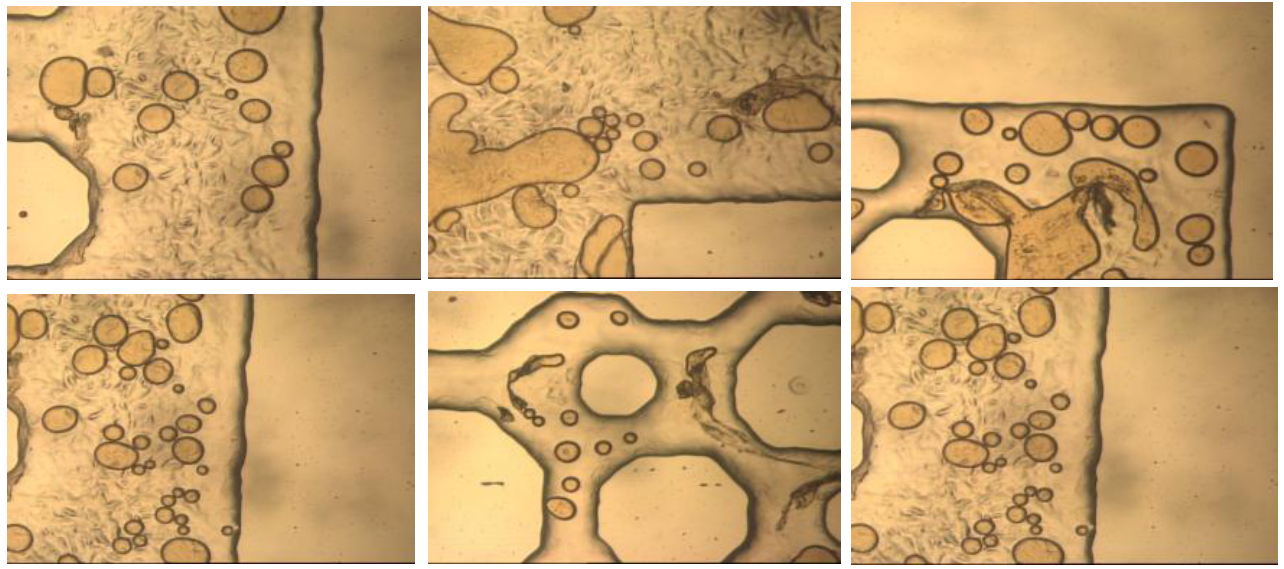
\includegraphics[width=\textwidth]{img/fig/microGlass.png}
    \caption{Visualization glass micromodel experiment with emulsions in higher concentration of nanoparticles. source: \citet{Li2013}}
    \label{fig:microGlass}
\end{figure}

In a later study, \citet{Hendraningrat2014} evaluated how the initial rock wettability would influence the ability of hydrophilic silica-based nanofluids to recover more oil. They used water-, intermediate-, and oil-wet systems with Berea sandstone in a temprature range of 25 - 80~\celsius. Their results showed that the effect of initial wettability was more dominant at higher temperatures. They also reported that using silica nanofluids they could reduce the residual oil saturation, improving oil recovery in all the three wettability cases, although best results were achieved in cased of the intermediate-wet system.   

\citet{Zargartalebi2015} examined whether anionic surfactant flooding would be enhanced in presence of hydrophilic and hydrophobic silica nanoparticles. Their results revealed that additoin of NPs affects the IFT between the oil and the surfactant as a function of NP concentration. The presence of NPs also reduced adsorption of surfactans on the rock surface, and this effect was more dominant with hydrophobic particles. Their subsequent core flooding resulted in improved oil recovery compared to conventional surfactant flooding.

\citet{Ye2013} studided the effect of nanoparticles in polymer flooding. They synthesized a copolymer by free radical polymerization of acrylamide (AM), acrylic acid (AA), and nano-SiO2 functional monomer (NSFM) as raw materials under mild conditions. Figure \ref{fig:AMAANP} shows the structural difference between the molecular chains of copolymer with and without nanoparticles. As illustrated in Figure \ref{fig:AM-AA-NP}, when nanoparticles were introduced the molecular chains of AM/AA/NSFM consisted of many micro-nano structure units. Their results indicated that this structure had higher apparent viscosity at 500 s$^{-1}$ shear rate, achieved up to 43.7\% viscosity retention rate at 95~\celsius, exhibited higher resistance factor and residual resistance factor resulting in better mobility control and higher oil recovery.
\begin{figure}
    \begin{subfigure}{\textwidth}
    \centering
    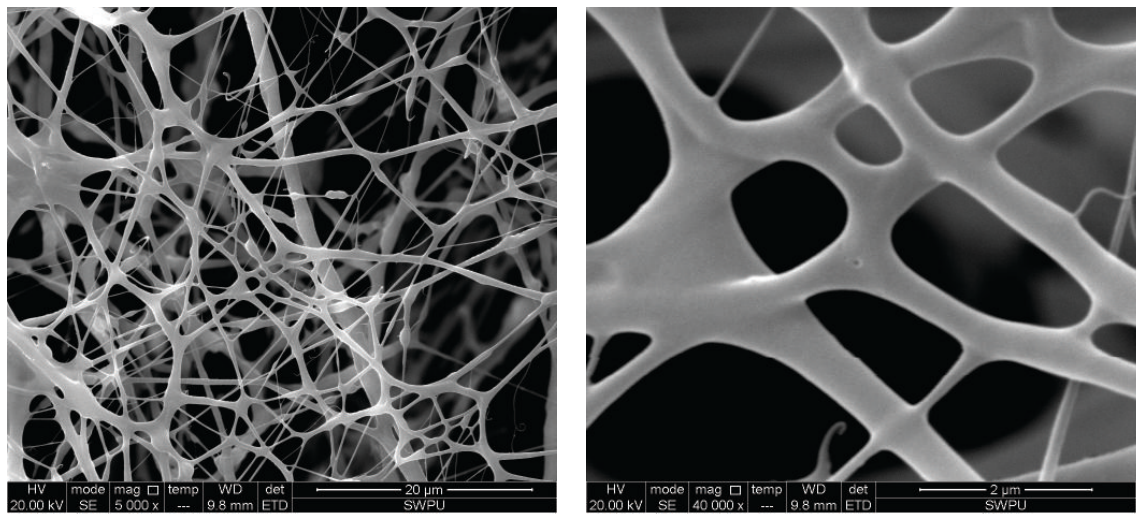
\includegraphics[width=\textwidth]{img/fig/AM-AA.png}
    \caption{SEM images of AM/AA at two magnification scales}
    \label{fig:AM-AA}
    \end{subfigure}
    \\
    \begin{subfigure}{\textwidth}
    \centering
    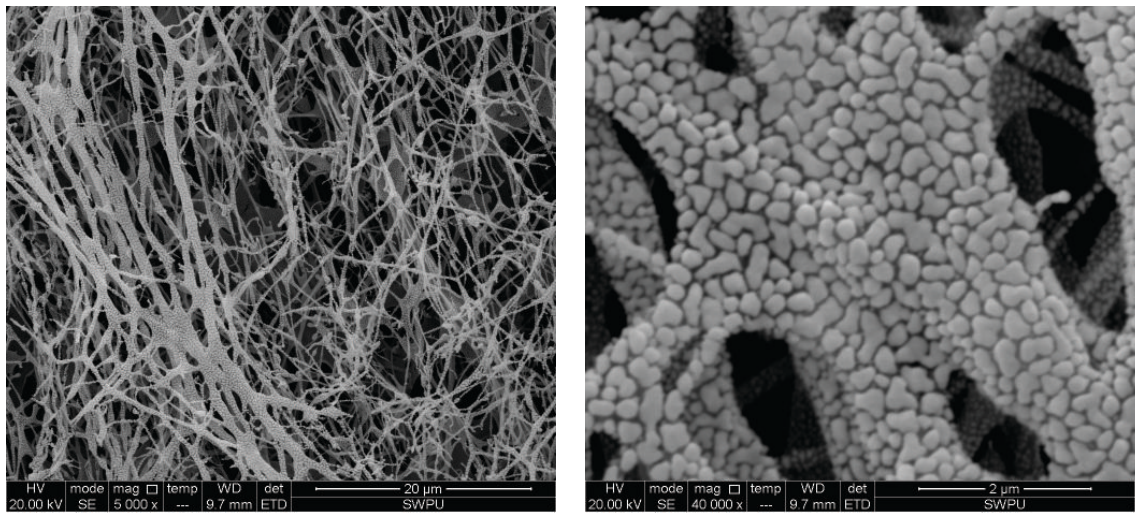
\includegraphics[width=\textwidth]{img/fig/AM-AA-NP.png}
    \caption{SEM images of AM/AA/NSFM at two magnification scales}
    \label{fig:AM-AA-NP}
    \end{subfigure}
    
    \caption{Comparison of the polymer structure of AM/AA with and without NSFM. source: \citet{Ye2013}}
    \label{fig:AMAANP}
\end{figure}    


\ce{CO2} based EOR methods face several challenges. One challenge is early gravity segregation of \ce{CO2} due to lower density compared to water, preventing \ce{CO2} from sweeping lower zones of the reservoir. Another challenge arises due to lower viscosity of \ce{CO2} leading to viscous fingering and early breakthrough of \ce{CO2} through the highly permeable channels in the reservoir. Therefore, in order to reap the benefits of \ce{CO2} injection for EOR, its mobility must be reduced, and the \ce{CO2} foam (gas in liquid colloid) must be stabilized. 

Nanoparticles have been the subject of various research studies on the foam stabilization front as well. \citet{Zhang2009} studied the application of nanoparticles in stabilizing foams under high temperature reservoir conditions. \citet{Manan2015} investigated the effects of different types of nanoparticles, namely silicon dioxide, aluminum oxide, copper oxide and titanium dioxide on stabilizing \ce{CO2} foams for mobility control in immiscible gas flooding. They concluded that low concentrations of nanoparticles can bring about high foam resistance and stability, with aluminum oxide particles performing best. \citet{Singh2016} could stabilize foam using surface-modified nanoparticles (SMNPs) both in bulk and porous media. They synthesized SMNPs by partial hydrophobization of alumina-coated silica nanoparticles with a surface modifier. More recently, \citet{Barrabino2018} experimentally compared the effect of graphene oxide, nanographene oxide and partially reduced graphene oxide on stabilizing \ce{CO2} foams. The results of their experiments revealed that nanographene oxide was not suitable for \ce{CO2} EOR purposes due to its hydrophilic nature which results in formation of hydrogels in presence of divalent ions and hinders their transport through porous media.

Some studies such as those carried out by \citet{HamediShokrlu2010, HamediShokrlu2013} have investigated the effect of nanoparticles on EOR methods that address heavy oil production by means of viscosity reduction Fand/or interfacial tension (IFT) modification. \citet{LI2007} used a nano-nickel catalyst to reduce the viscosity of Liaohe extra-heavy oil by aqua-thermolysis\footnote{\citet{Hyne1986} defines aqua-thermolysis as the interaction of high-pressure/high-temperature water steam with the reactive components of heavy oil and bitumen}. They could successfully upgrade the heavy oil through aqua-thermolysis whereby some of C-S bonds in the extra-heavy oil were broken and the mean molar weight of the heavy oil was reduced. \citet{Alomair2015} reported that right concentration of metal oxide nanoparticles can reduce viscosity and modify IFT for enhanced recovery of heavy oils. Based on their experimental study, silicon oxide (\ce{SiO2}) and aluminum oxide (\ce{Al2O3}) nanofluids yielded superior results than their counterparts, nickle oxide (\ce{NiO}) and titanium oxide (\ce{TiO2}). A mixture of \ce{SiO2}/\ce{Al2O3} with formation water gave the highest oil recovery in their study. They also observed the microscopic structure of said nanoparticles magnified to 25000X with a field emission scanning electron microscope (FESEM), as shown in Figure \ref{fig:npFesem}.


\begin{figure}
    \centering
    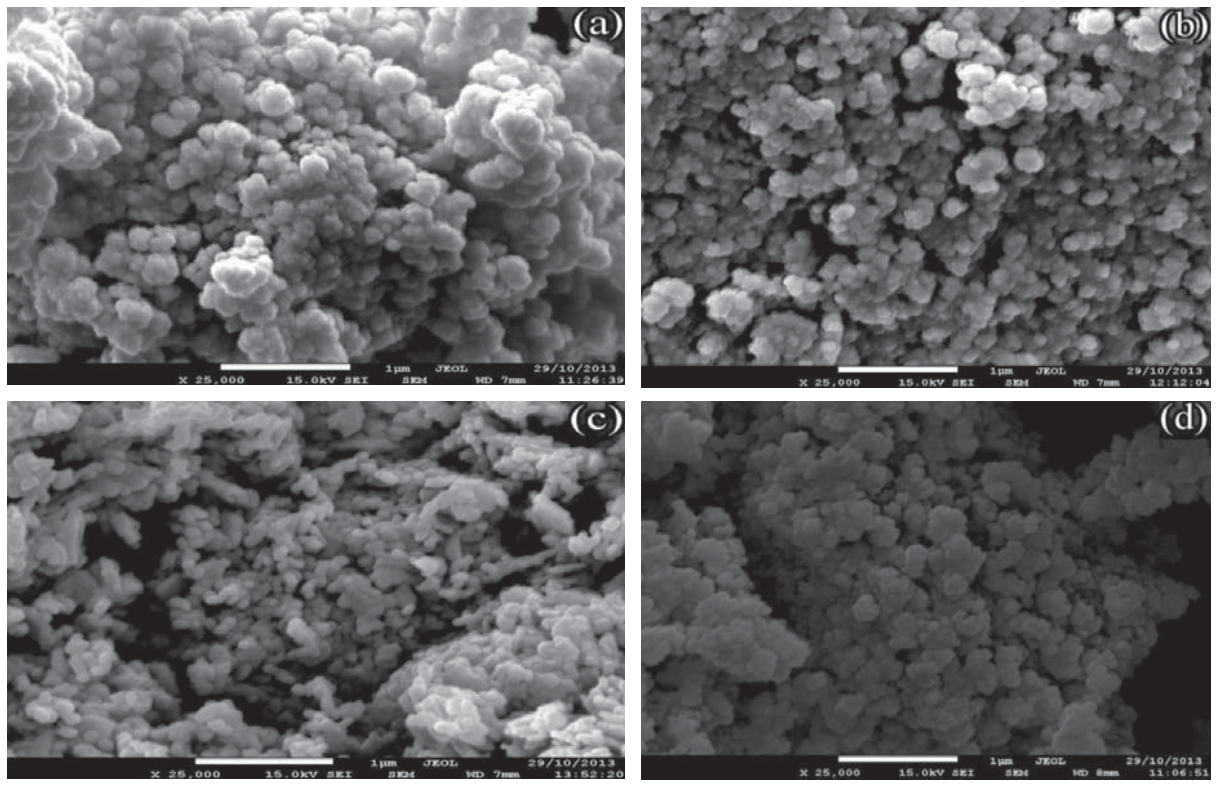
\includegraphics[width=\textwidth]{img/fig/npFesem.png}
    \caption{FESEM images of (a) titanium oxide, (b) aluminum oxide, (c) nickel oxide, and (d) silicon oxide. source: \citet{Alomair2015} }
    \label{fig:npFesem}
\end{figure}
















\section{Nanogels from polyelectrolyte complexes}


\section{Transport of polymer and nanoparticles in porous media}
The transport of water additives in porous media is governed by the phenomena retention, adsorption and inaccessible pore volume (IPV) as described by \citep{Lotsch1985}. Changes in composition of the injected solution (e.g., polymer, nanoparticles, salt concentration) affect the responses measured by various sensors. Figure 5.1 shows a few idealized cases of such responses. An ideal piston-like plug flow would look like a step function. However, the real-world effect from dispersion reforms the step function into a curve.

Inaccessible pore volume and retention can shift the curve in Figure \ref{fig:ipvRet1}. The portion of the porous media that cannot be accessed by the particle under study (e.g., the polymer) is referred to as inaccessible pore volume (IPV). The reduced accessible pore volume results in a faster transport of the particles across the porous medium and therefore shifts the response curve to the left. On the other hand, some of the particles under study can be adsorbed on the surface of the rock (adsorption) or are stuck and filtered in small pore throats (mechanical entrapment). These effects delay particle flow through porous media, which are collectively referred to as retention. As a result, the response curve is shifted to the right. 

One should only expect the effect of dispersion on responses for step changes in the salt concentration. However, polymer and nanoparticle responses can experience any combination of effects from dispersion, IPV, retention, and flooding history.

\begin{figure}[h!]
    \centering
    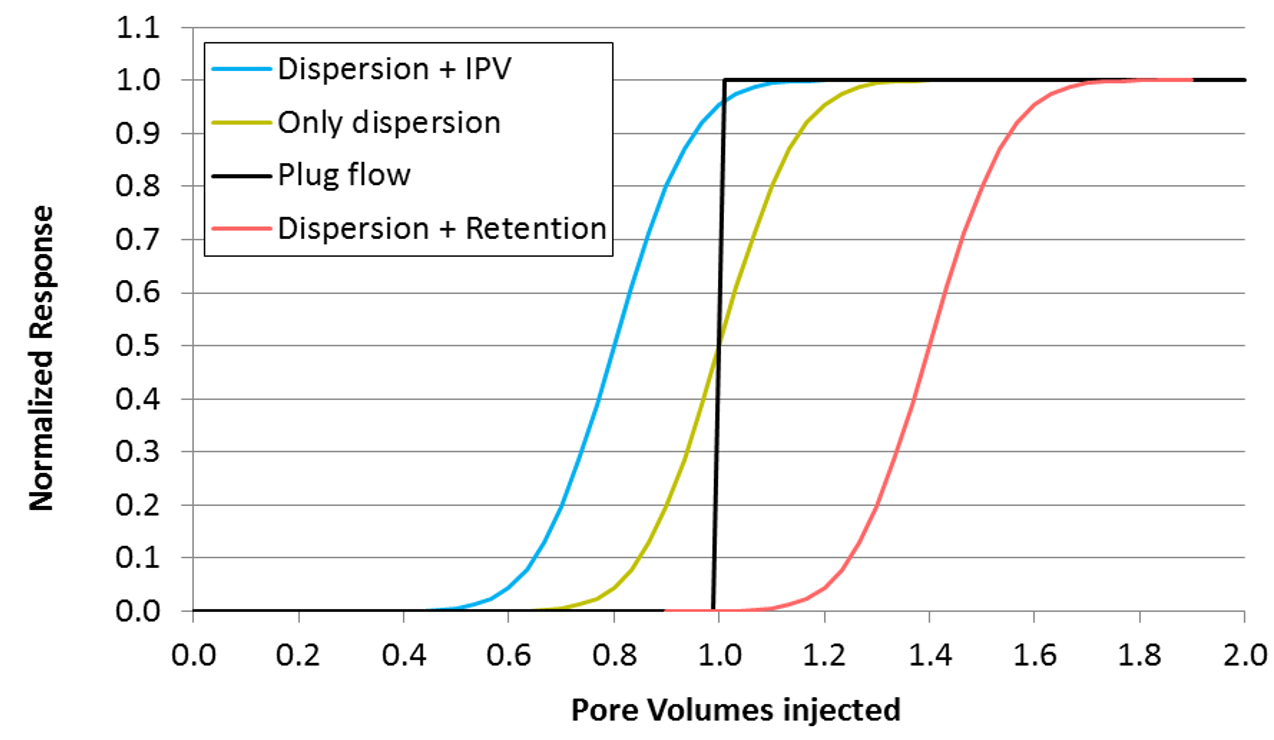
\includegraphics[width=\textwidth]{img/fig/ipvRet1.png}
    \caption{Effect of dispersion, inaccessible pore volume (IPV) and retention on relative responses.}
    \label{fig:ipvRet1} % 5.1
\end{figure}

In order to determine inaccessible pore volume of e.g., polymer, one can compare the production profiles of polymer and a tracer as a function of pore volumes injected. Figure \ref{fig:ipvRet2} illustrates such a comparison. The relative response of polymer is the ratio of measured effluent concentration to the injected concentration. The tracer should ideally have no IPV, i.e., the area below the tracer response should be equal to one. Changing the concentration in salt tracer will yield a close enough response. The area between the two responses determines the IPV.

\begin{figure}[h!]
    \centering
    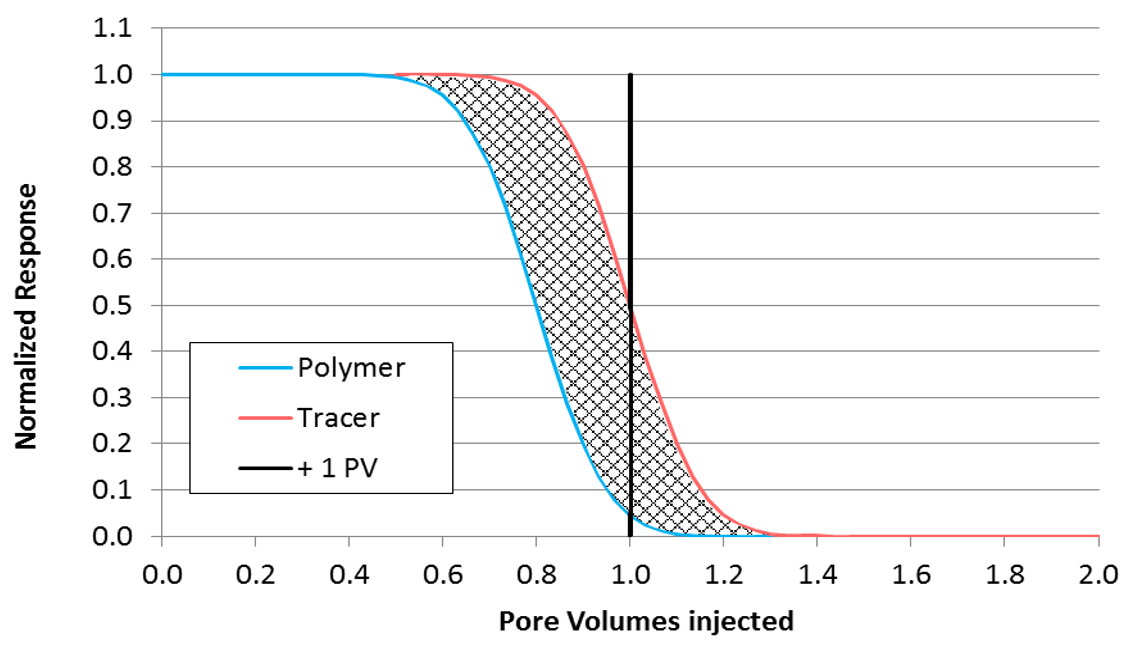
\includegraphics[width=\textwidth]{img/fig/ipvRet2.png}
    \caption{Effect of dispersion, inaccessible pore volume (IPV) and retention on relative responses.}
    \label{fig:ipvRet2} % 5.2
\end{figure}

Provided that the adsorption of polymer is irreversible and no mechanically entrapped polymer is released during water injection, the IPV will result in a response curve with an area under the curve of less than 1. Thus, IPV for polymer will be a positive value. However, if the system experiences desorption of the mechanically entrapped component, the area under the curve may become larger than the tracer area, resulting in a negative IPV indicating release of retained component. 

Total retention of a component in the rock depends on adsorption and mechanical entrapment. A multi-slug experiment can be used to quantify adsorption. Assuming that adsorption for the component under study were irreversible, all the adsorption happened in the first slug, i.e., no more adsorption took place during the second slug, and the magnitude of mechanical entrapment in both slugs were equal, one can compare the relative responses from the two slugs to find adsorption for the component. This is illustrated in Figure \ref{fig:ipvRet3}.

\begin{figure}[h!]
    \centering
    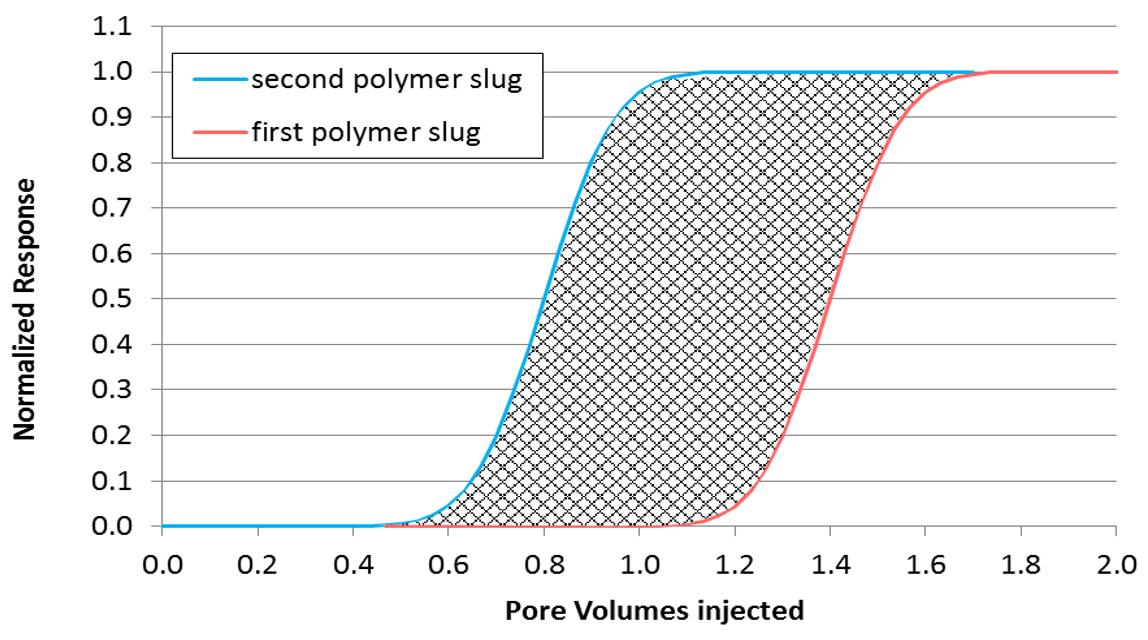
\includegraphics[width=\textwidth]{img/fig/ipvRet3.png}
    \caption{Effect of dispersion, inaccessible pore volume (IPV) and retention on relative responses.}
    \label{fig:ipvRet3} % 5.3
\end{figure}